\documentclass[9pt]{beamer}
\usepackage[utf8]{inputenc}
\usepackage[T1]{fontenc}
\usepackage[russian]{babel}
\usepackage{graphicx}
\usepackage{tikz}
\usepackage{pifont}
\usetheme{Dresden}
\usecolortheme{beaver}
\setbeamerfont{block title}{size=\normalsize}
\beamertemplatenavigationsymbolsempty
\title[Electric motors data analysis]{\huge Electric motors data analysis}
\author[Snesarevskii, Belli, Biava, Dragi\'c, Kalenova] {{\Large Group 8:\\}Viktor Snesarevskii\\Edoardo Belli\\Guendalina Biava\\Ozrenka Dragi\'c\\Madina Kalenova}
\date{March-April 2018}

\begin{document}
	\begin{frame}
	\titlepage
	\vfill
	\begin{flushright}
		
\includegraphics[height=.7cm]{abb.png}
	\end{flushright}
\end{frame}

\begin{frame}{Dataset}
\begin{itemize} %[<+->]
\item Measurements of torque and current from electric motors
\item Time-series data with frequency 20KHz (downsampled by a factor \textit{M=100} for real use cases/ease of computation)
\item Data taken from 5 distinct motors in AC and DC modes
\item Each data sample is one recorded operation
\item Operations are recorded while the motor is working properly, then a fault is induced and the same operations are recorded again 
\item 1066 AC samples, 924 DC samples (focusing on the DC for now)
\end{itemize}
\end{frame}

\begin{frame}{The Dataset}
\centering
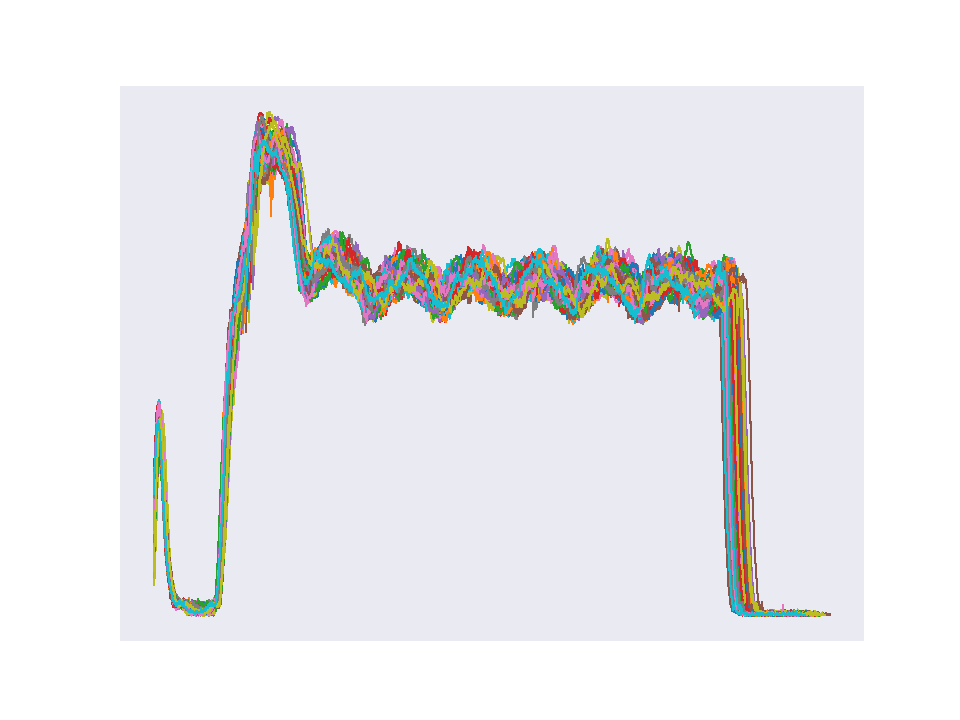
\includegraphics[width=0.85\textwidth]{multiplot.pdf}
\end{frame}

\begin{frame}{Exploratory Analysis: First Approach}
\begin{itemize} %[<+->]
\item {\large Feature Extraction}\\
Choose a set of features and check if they are statistically significant for the underlying problem ---> to be used later in classification
\item {\large Our set of features is:}\\
Mean, Standard Deviation, Mode, Median
\end{itemize}
\end{frame}

\begin{frame}{Scatterplot --- Currents, Binary}
\centering
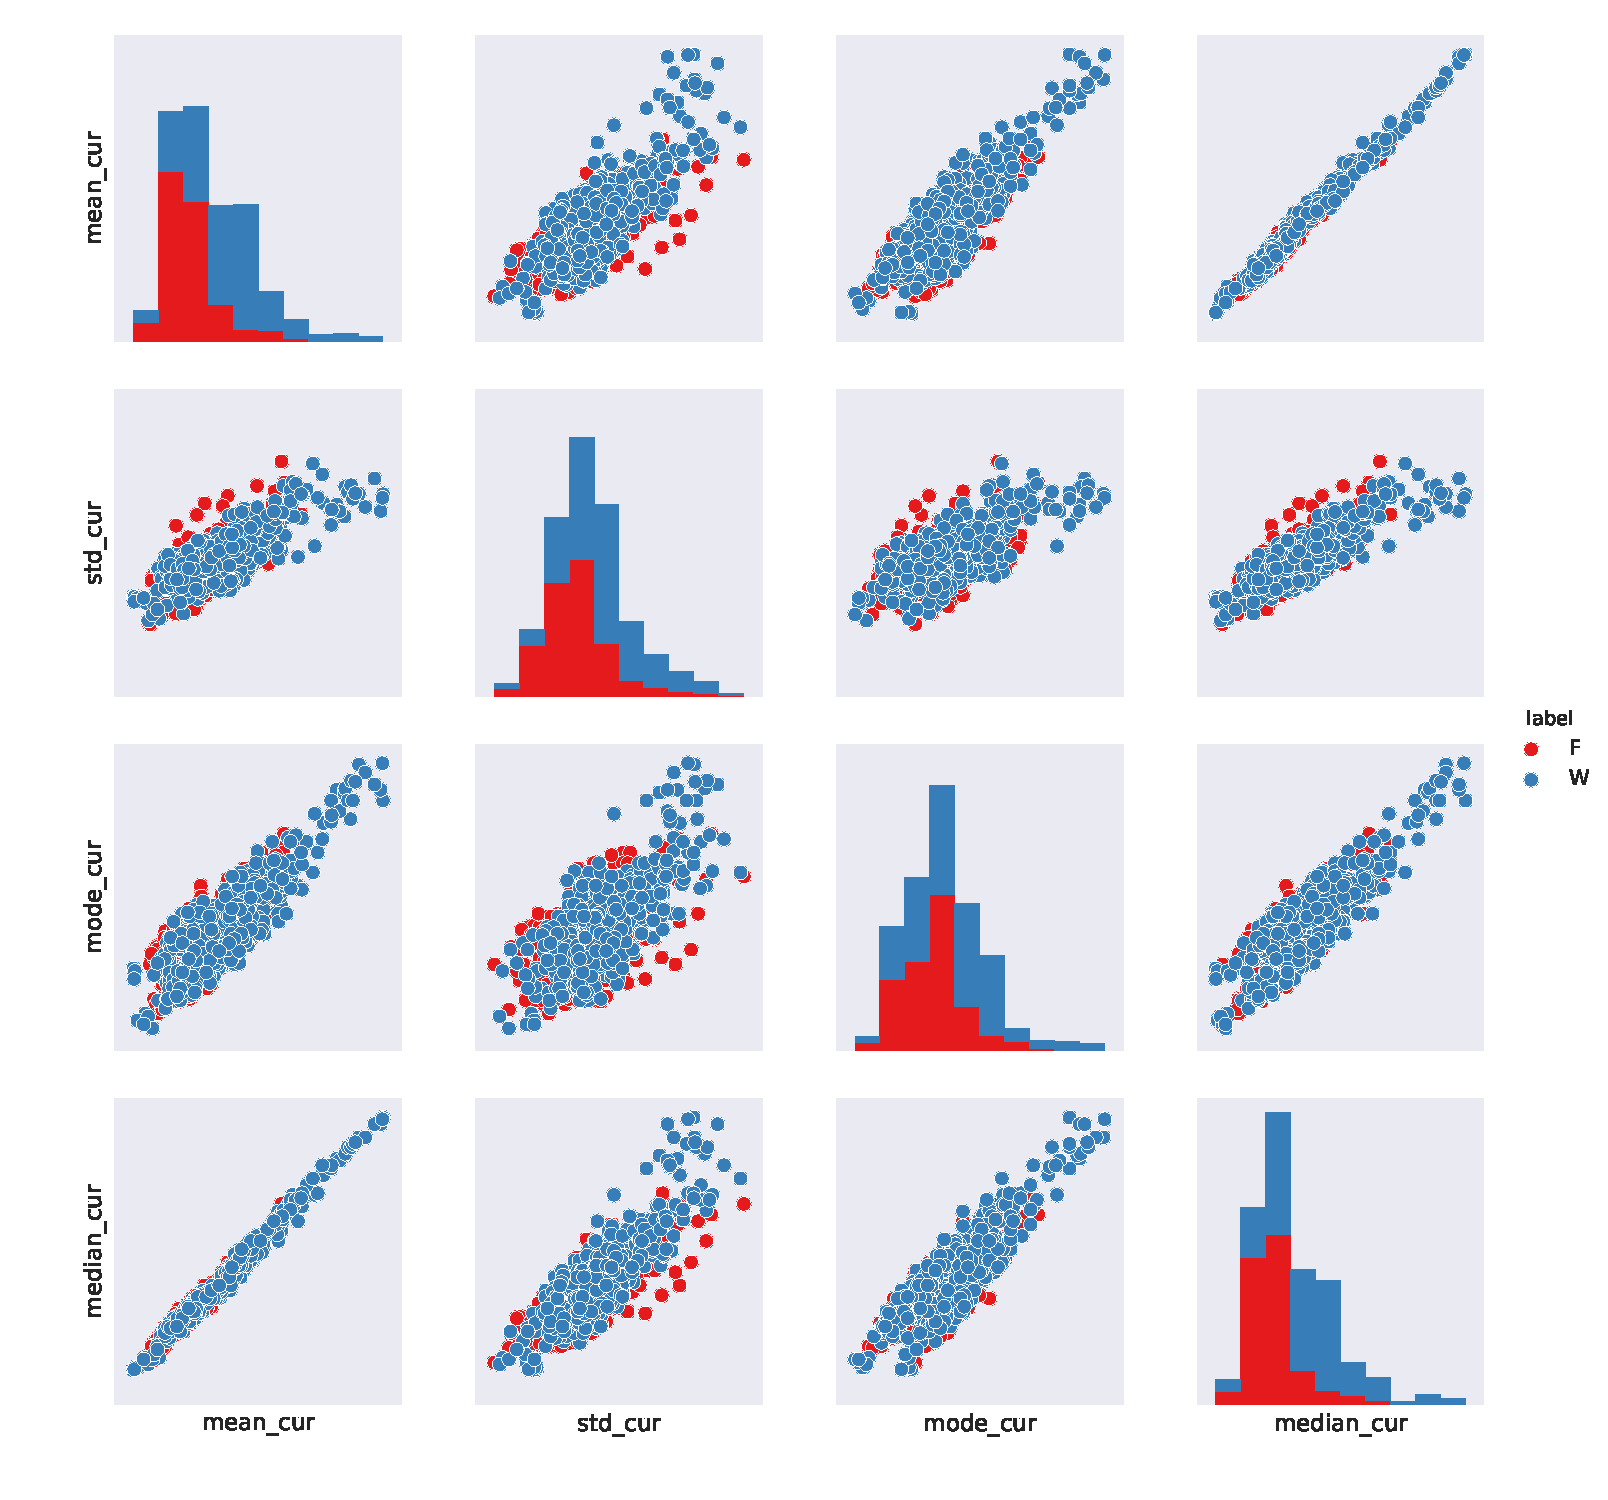
\includegraphics[width=0.75\textwidth]{scattermatrix_currents_bin.pdf}
\end{frame}

\begin{frame}{Scatterplot --- Torques, Binary}
\centering
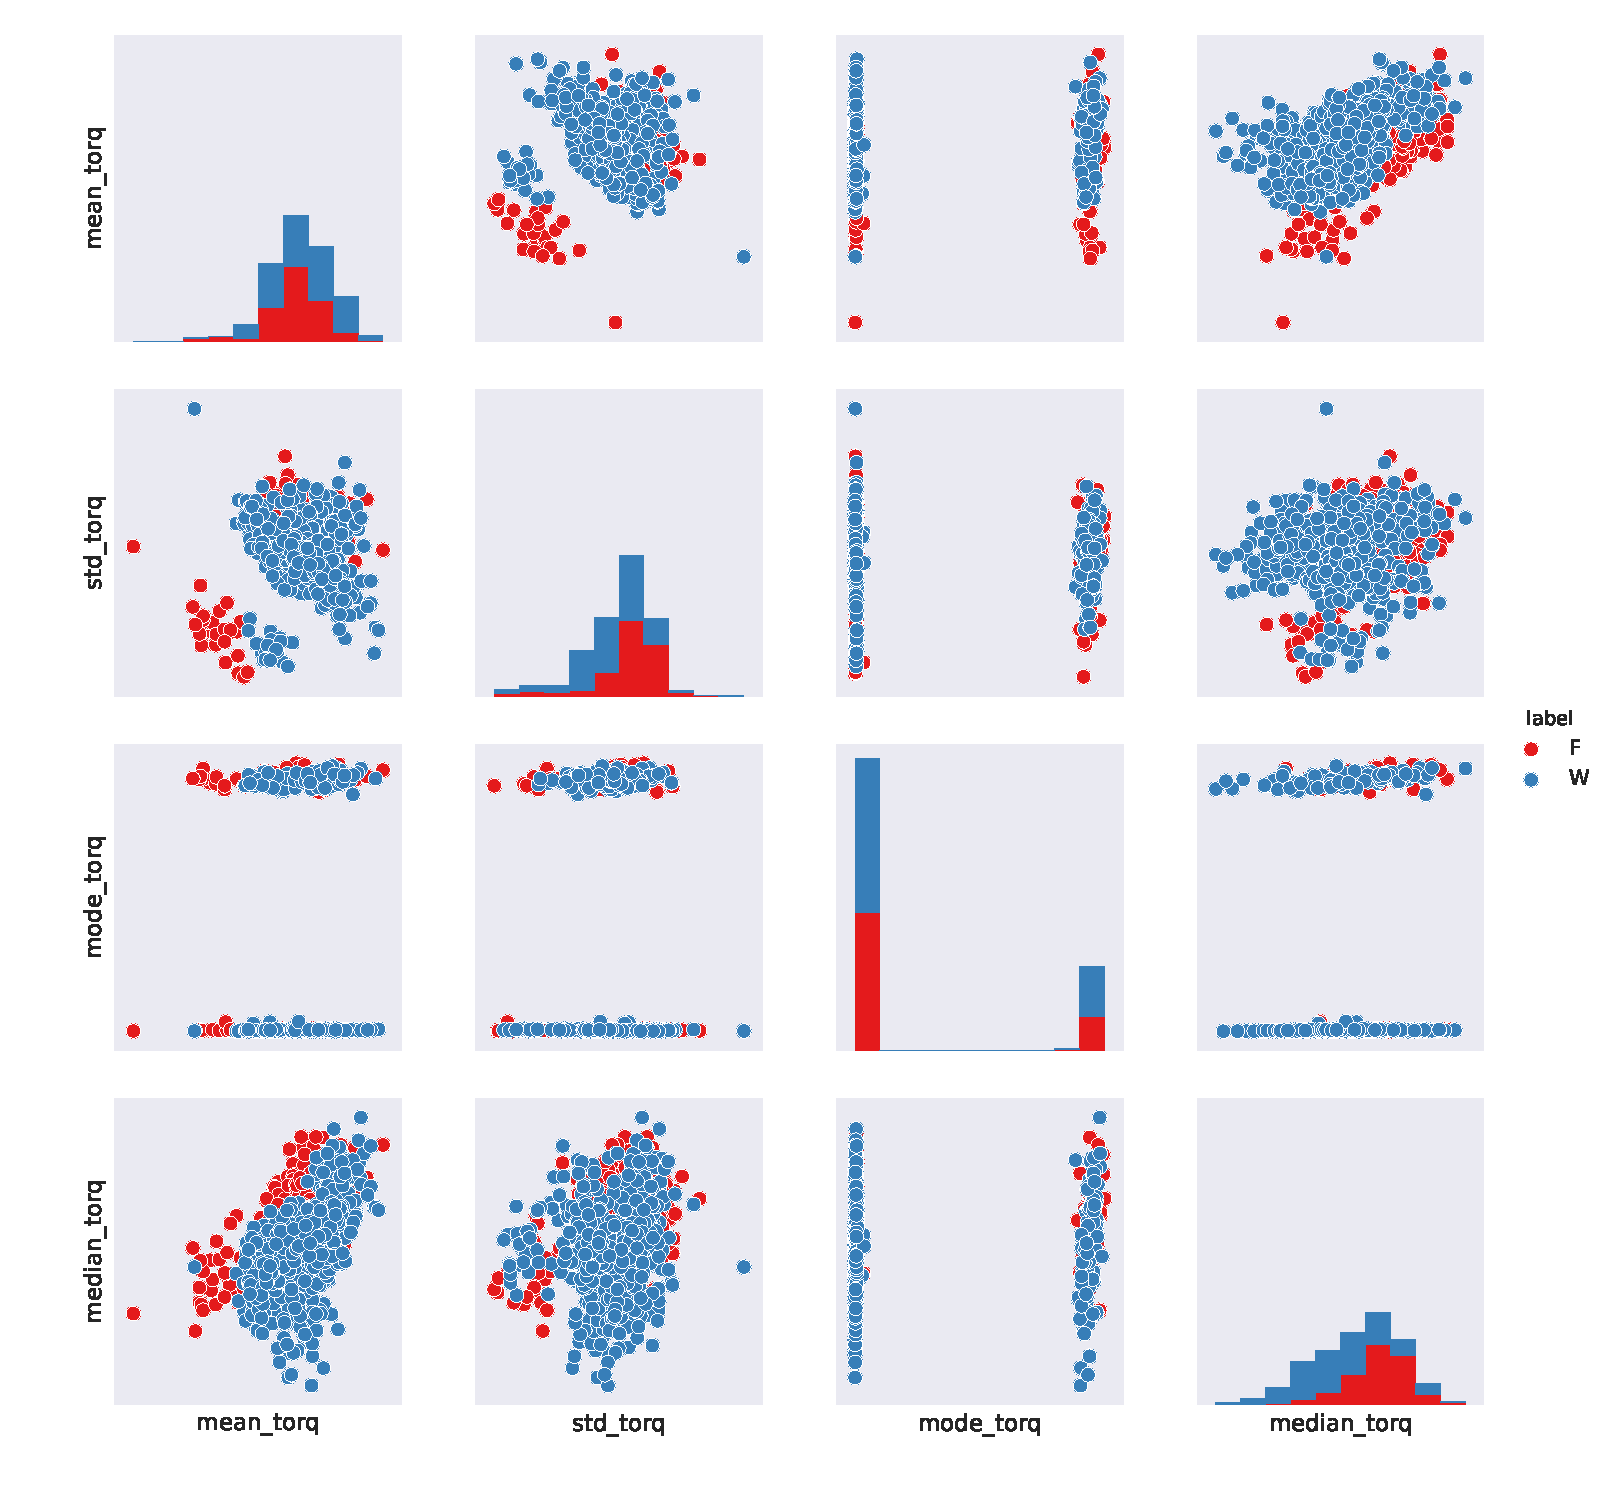
\includegraphics[width=0.75\textwidth]{scattermatrix_torques_bin.pdf}
\end{frame}

\begin{frame}{Scatterplot --- Currents, Multiclass}
\centering
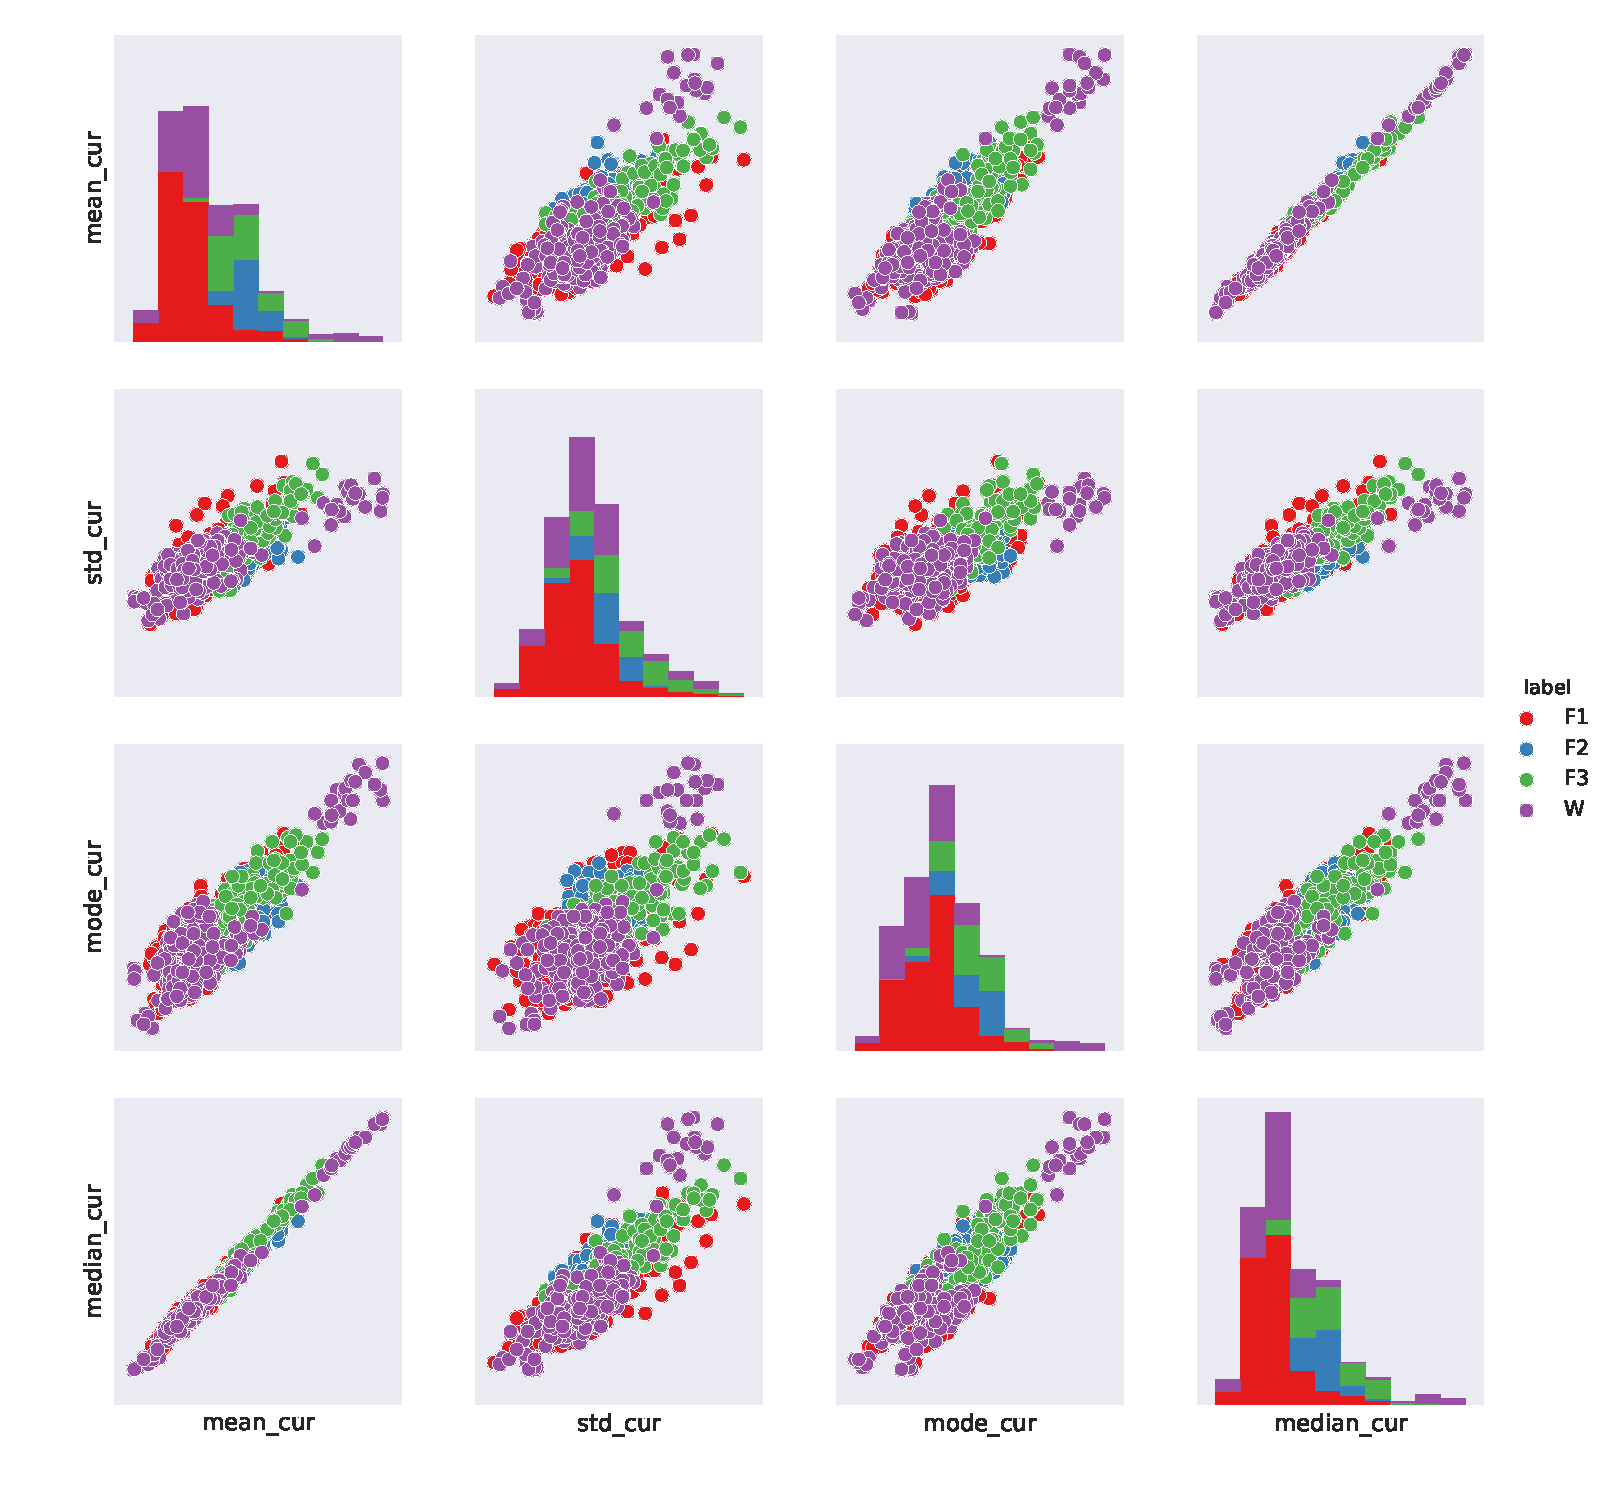
\includegraphics[width=0.75\textwidth]{scattermatrix_currents_multi.pdf}
\end{frame}

\begin{frame}{Scatterplot --- Torques, Multiclass}
\centering
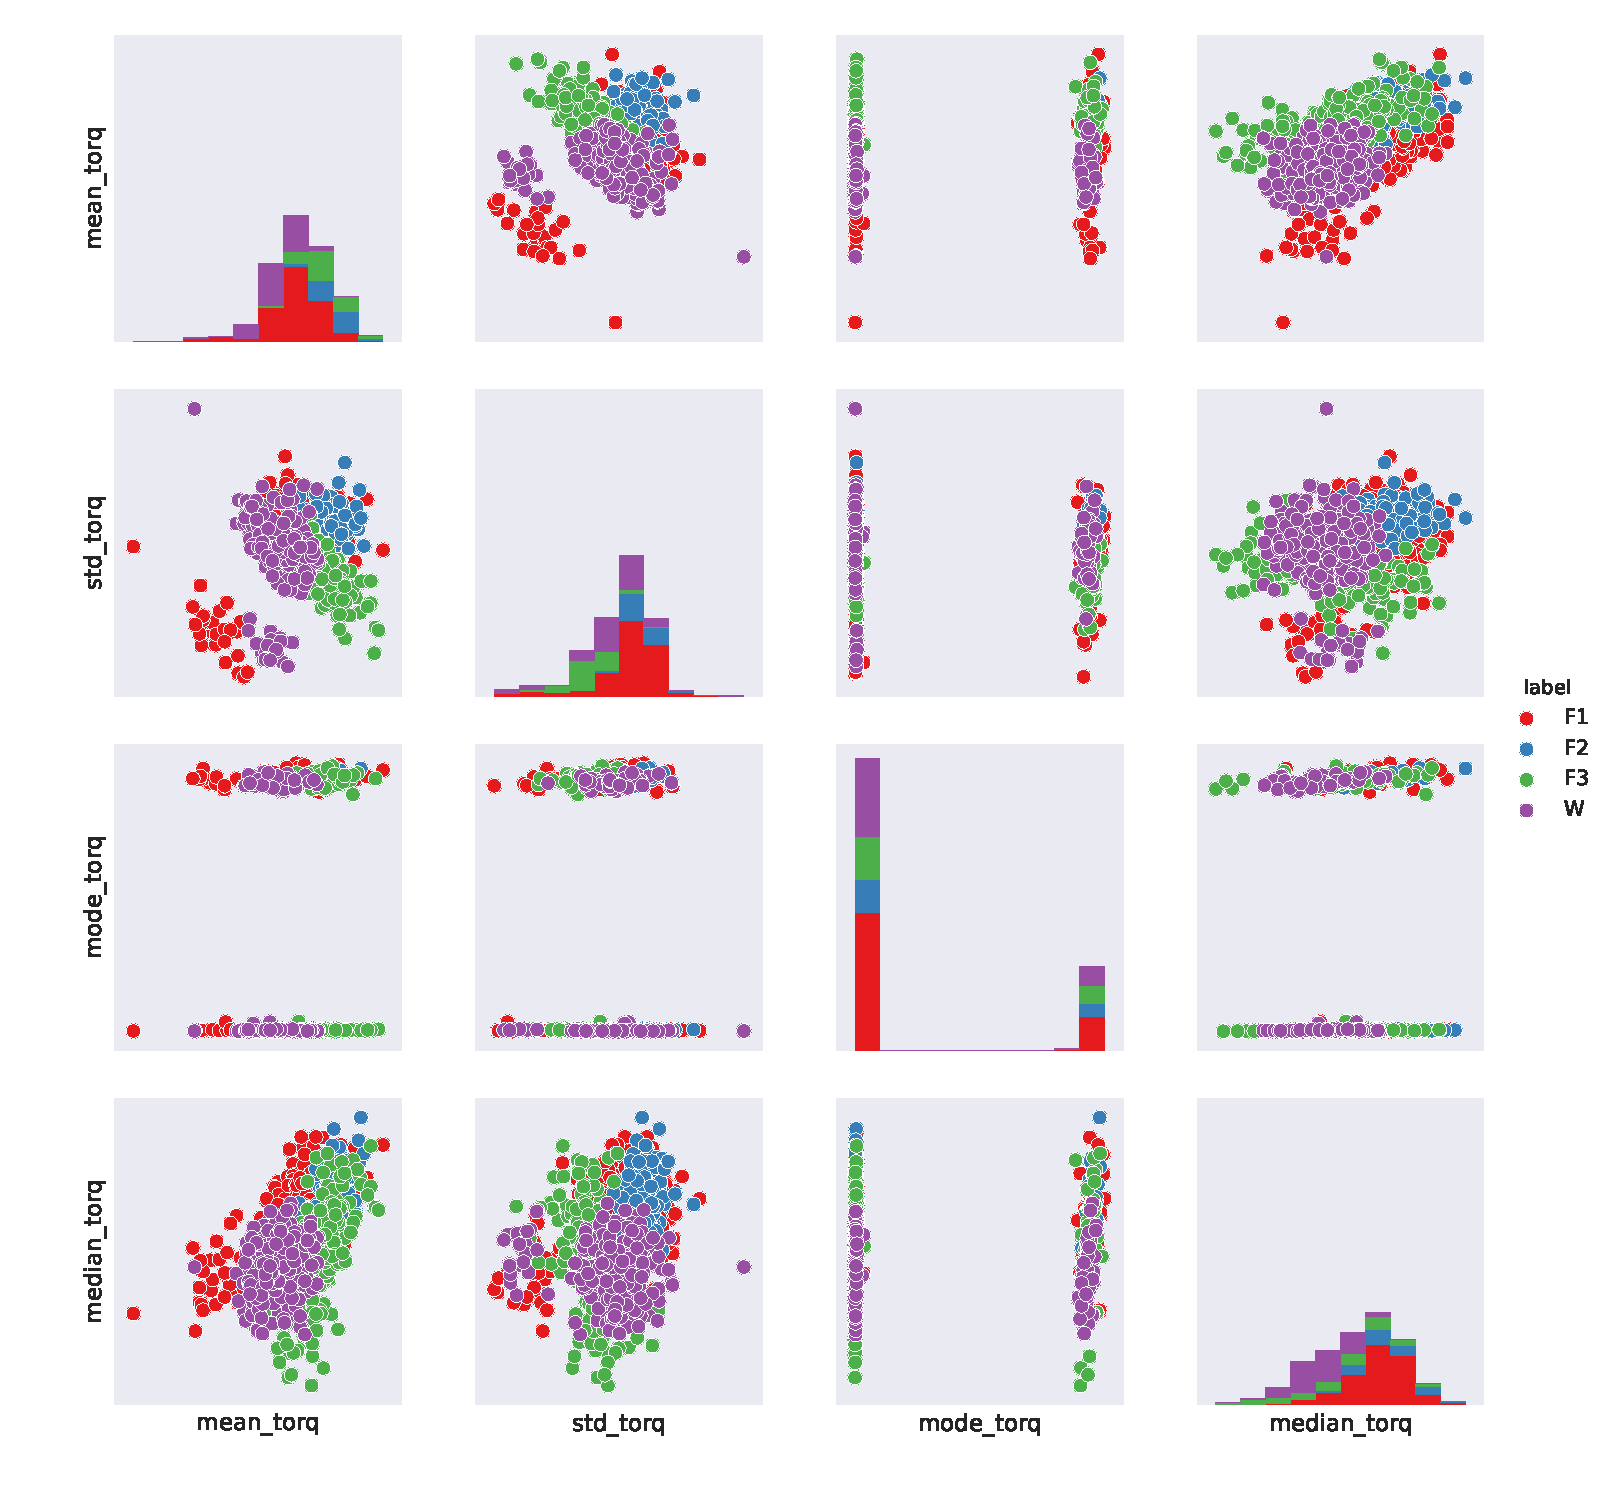
\includegraphics[width=0.75\textwidth]{scattermatrix_torques_multi.pdf}
\end{frame}

\begin{frame}{Exploratory Analysis: Second Approach}
\begin{itemize} %[<+->]
\item {\large Principal Component Analysis (time-series data, \textit{p=1524})}\\
Identify the measurement times where we have maximum variability ---> to be used later for classification/prediction
\end{itemize}
\end{frame}

\begin{frame}{Principal Component Analysis: Currents, \textit{p=1524, N=924}}
\centering
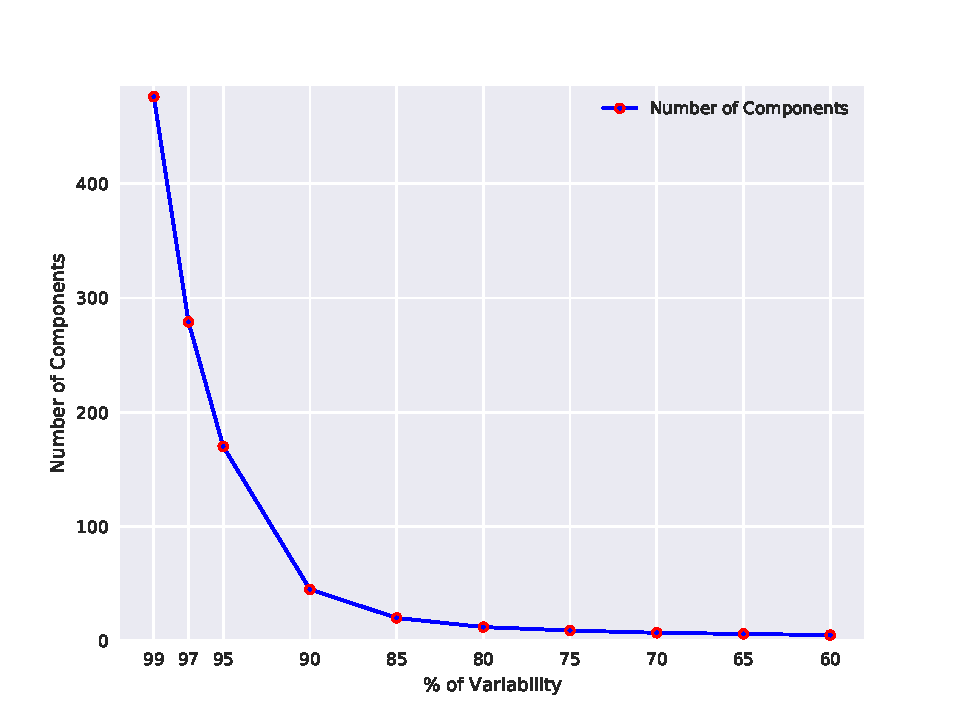
\includegraphics[width=0.85\textwidth]{n_pc_curr.pdf}
\end{frame}

\begin{frame}{Principal Component Analysis: Torques, \textit{p=1524, N=924}}
\centering
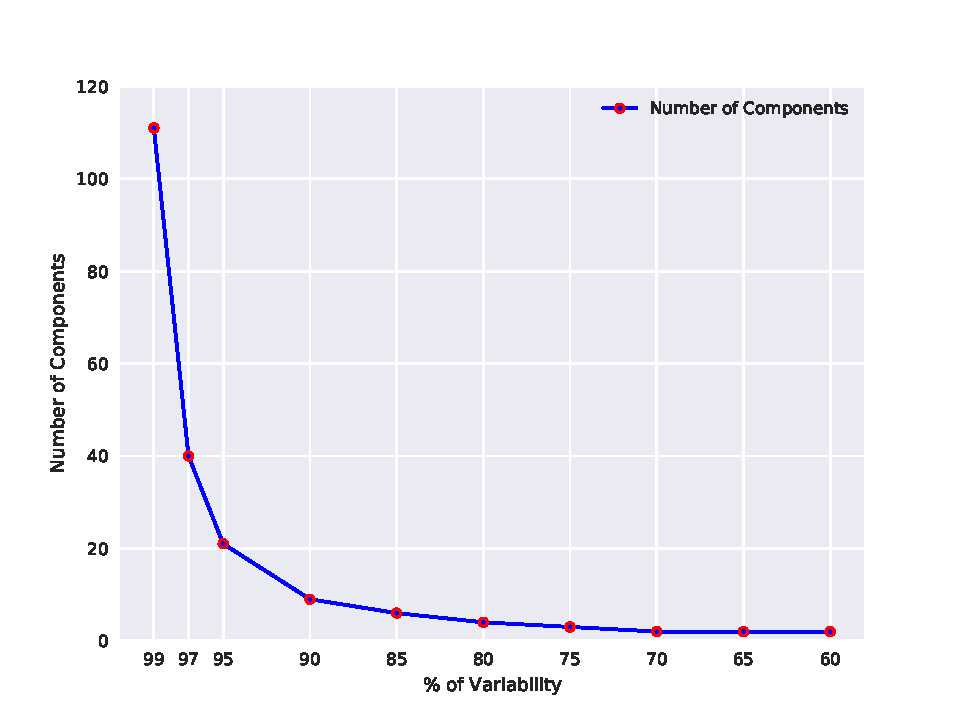
\includegraphics[width=0.85\textwidth]{n_pc_torq.pdf}
\end{frame}

\begin{frame}{Final Goals}
ABB is interested in three main applications:
\begin{itemize} %[<+->]
\item {\large Motor Classification}\\
Can we identify a motor by a recorded operation?
\item {\large Fault Classification}\\
Can we group motors by their state (working/faulty)?
\item {\large Fault Prediction}\\
Can we predict the state of a motor by measuring current and torque during an operation?
\end{itemize}
\end{frame}

\begin{frame}{Conclusions}
\begin{itemize} 
\item {\large First Approach}\\
Further improvements can be made by adding different features and/or transforming the input data, the current feature set doesn't show a clear separation between faulty and working motors.
\item {\large Second Approach}\\
Most of the variability can be captured with a relatively low number of components (10/20 vs p=1524).
\end{itemize}
\end{frame}

\end{document}